\chapter{Tutorial Remove C-Comment ( C )}

\section{Scope}

In this tutorial you will create a more complex model. The model implements a simple parser that removes comments (block comments and line comments) from a C source file. Therefore we will create two actors. One actor is responsible to perform the file operations, while the second actor implements the parser.

You will perform the following steps:

\begin{enumerate}
\item create a new model from scratch for C
\item define a protocol
\item define your own data type
\item create the structure and the behavior by yourself
\item generate, build and run the model
\end{enumerate}

Make sure that you have set up the workspace as described in \textit{Setting up the Workspace for C Projects}.

\section{Create a new model from scratch}

Remember the following steps from the previous tutorials:
\begin{itemize}
\item select the \textit{C/C++} perspective
\item From the main menue select \textit{File->New->C Project}
\item Name the project \textit{RemoveComment}
\item Project type is \textit{Executable / Empty C Project}
\item Toolchain is \textit{MinGW}
\item Add the folder \textit{model}
\item Add the model file and name it \textit{RemoveComment.room}
\item Add the Xtext nature.
\end{itemize}

The workspace should look like this:

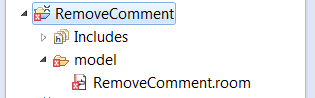
\includegraphics{images/036-RemoveCommentC01.png}
% !images/036-RemoveCommentC01.png!

Create a launch configuration for the C generator and add the include path and library as described in \textit{HelloWorldC}.

The workspace should look like this:

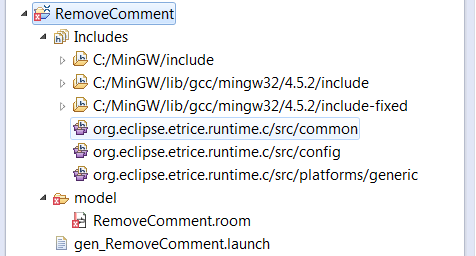
\includegraphics{images/036-RemoveCommentC02.png}
% !images/036-RemoveCommentC02.png!

Now the model is created and all settings for the code generator, compiler and linker are done.


\section{Create your own data type}

The planed application should read a C source file and remove the comments. Therefore we need a file descriptor which is not part of the basic C types. The type for the file descriptor for MinGW is \textit{FILE}. To make this type available on the model level, you have to declare the type. 

Open the file \textit{Types.room} from \textit{org.eclipse.modellib.c} and take a look at the declaration of \textit{string} (last line) which is not a basic C type.

\textit{PrimitiveType string:ptCharacter -> charPtr default "0"}

With this declaration, you make the \textit{string} keyword available on model level as a primitive type. This type will be translated to \textit{charPtr} in your C sources. \textit{charPtr} is defined in \textit{etDatatypes.h}. This header file is platform specific (\textit{generic}). With this mechanism you can define your own type system on model level and map the model types to specific target/platform types. 

To not interfere with other models, we will declare the type direct in the model.
Add the following line to your model:

\begin{small}
\begin{verbatim}
RoomModel RemoveComment {
	import room.basic.types.* from 
		"../../../org.eclipse.etrice.modellib.c/model/Types.room"
	
	PrimitiveType file:ptInteger -> FILE default "0"
\end{verbatim}
\end{small}

\textit{FILE} is the native type for MinGW. Therefore you don't need a mapping within \textit{etDatatypes.h}. If your model should be portable across different platforms you should not take this shortcut.
 
\section{Create the model}

Due to the former tutorials you should be familiar with the steps to create the model with protocols, actors and state machines.

The basic idea of the exercise is to create a file reader actor, which is responsible to open, close and read characters from the source file. Another actor receives the characters and filters the comments (parser). The remaining characters (pure source code) should be print out. 

Remember the logical steps: 
\begin{itemize}
\item create the model by the help of content assist (CTRL Space)
\item name the model, subsystem and top level actor
\item define the protocol (in this case it should be able to send a char, and to request the next char from the file reader)
\item create the structure (file reader and parser with an appropriate port, create the references and connect the ports)
\item create the state machines
\end{itemize}

Try to create the model by yourself and take the following solution as an example.

Structure:

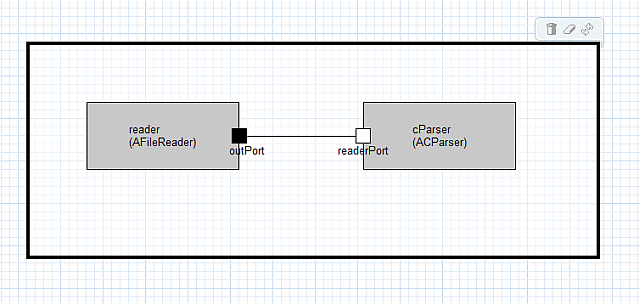
\includegraphics[width=\linewidth]{images/036-RemoveCommentC04.png}
% !images/036-RemoveCommentC04.png!

File reader FSM:

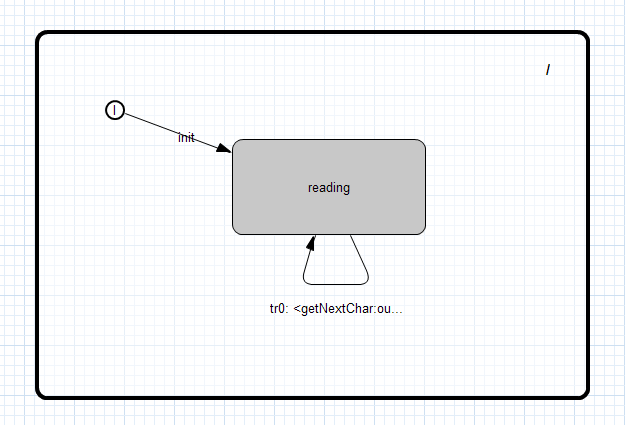
\includegraphics[width=\linewidth]{images/036-RemoveCommentC05.png}
% !images/036-RemoveCommentC05.png!

Parser FSM:

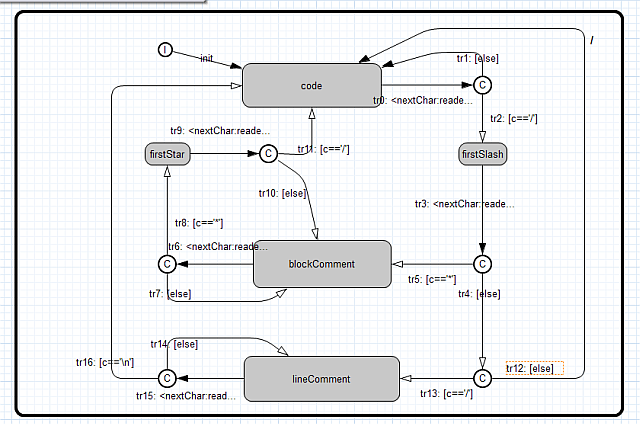
\includegraphics[width=\linewidth]{images/036-RemoveCommentC06.png}
% !images/036-RemoveCommentC06.png!

The complete model can be found in \textit{org.eclipse.etrice.tutorials.c}

Take a look at the file attribute of the file reader. 

\begin{verbatim}
Attribute f:file ref
\end{verbatim}

\textit{fopen} expects a \textit{FILE *}. \textit{f:file ref} declares a variable \textit{f} from type reference to \textit{file}, which is a pointer to \textit{FILE}.


\section{Generate, build and run the model}

Before you can run the model you should copy one of the generated C source files into the project folder and name it \textit{test.txt}. 

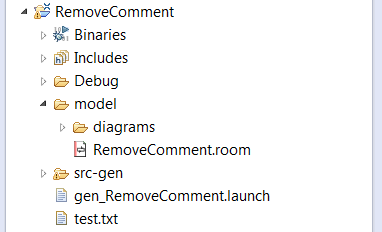
\includegraphics{images/036-RemoveCommentC07.png}
% !images/036-RemoveCommentC07.png!

Generate, build and run the model.

Your output should start like this:

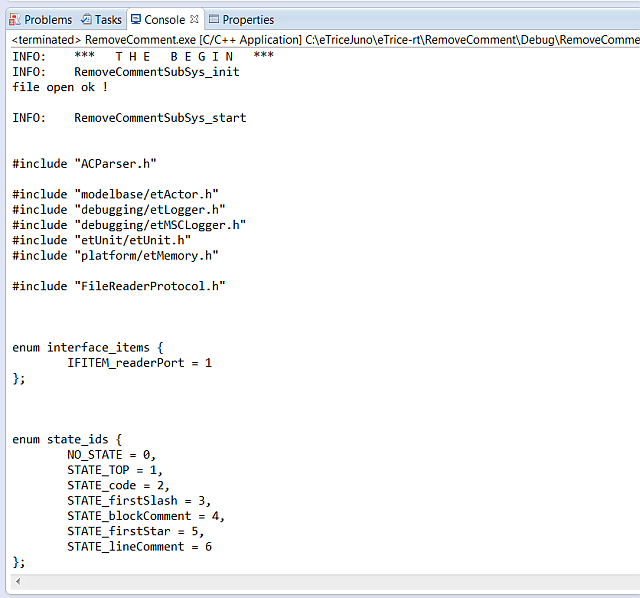
\includegraphics[width=\linewidth]{images/036-RemoveCommentC08.png}
% !images/036-RemoveCommentC08.png!


\section{Summary}

This tutorial should help you to train the necessary steps to create a C model. By the way you have seen how to create your own type system for a real embedded project. An additional aspect was to show how simple it is to separate different aspects of the required functionality by the use of actors and protocols and make them reusable.
